%%%%%%%%%%%%%%%%%%%%%%%%%%%%%%%%%%%%%%%%
\begin{frame}
  \frametitle{Road Map}
\begin{block}{CI for Normal Mean ($\sigma$ known)}
  \vspace{-1em}
  \[\bar{X}_n \pm \texttt{qnorm}(1-\alpha/2) \times \sigma/\sqrt{n}\]
\end{block}

\begin{block}{Assumptions Used}
	\begin{enumerate}
\item Population standard deviation $\sigma$ is known.
\item Population is normally distributed (bell-shaped).
\end{enumerate}
\end{block}

\begin{block}{What if the assumptions are wrong?}
\begin{enumerate}
  \item Population is normally distributed but $\sigma$ is unknown
  \item \alert{Population isn't normally distributed}
\end{enumerate}
\end{block}

\end{frame}
%%%%%%%%%%%%%%%%%%%%%%%%%%%%%%%%%%%%%%%%
\begin{frame}
\frametitle{We Don't know $\sigma$. What to use instead?}
$$\boxed{\bar{X}_n \pm \texttt{qnorm}(1-\alpha/2) \times \sigma/\sqrt{n}}$$

\begin{block}{What about Sample Standard Deviation $S$?}
	$$P\left(-2 \leq \frac{\bar{X}_n-\mu}{S/\sqrt{n}} \leq 2 \right) = 0.95 \mbox{ ???}$$
\end{block}

\begin{block}{Not Quite!}
Although $(\bar{X}_n-\mu)/(\sigma/\sqrt{n})\sim N(0,1)$, $S \neq \sigma$. In fact, $S$ is an \alert{estimator} of $\sigma$ so it is a \alert{random variable!}
\end{block}
\end{frame}
%%%%%%%%%%%%%%%%%%%%%%%%%%%%%%%%%%%%%%%%
\begin{frame}
\frametitle{Punchline: Sampling Distribution of $\sqrt{n}(\bar{X}_n-\mu)/S$}
If $X_1, \hdots, X_n \sim \mbox{iid } N(\mu,\sigma^2)$, then
	$$\alert{\boxed{\frac{\bar{X}_n - \mu}{S/\sqrt{n}} \sim t(n-1)}}$$
\end{frame}
%%%%%%%%%%%%%%%%%%%%%%%%%%%%%%%%%%%%%%%%
\begin{frame}
\frametitle{Who was ``Student?''}
\framesubtitle{\href{http://www.aeaweb.org/articles.php?doi=10.1257/jep.22.4.199}{\fbox{``Guinnessometrics: The Economic Foundation of Student's t''}}}

\begin{columns}

\column{0.3\textwidth}
\begin{figure}
\fbox{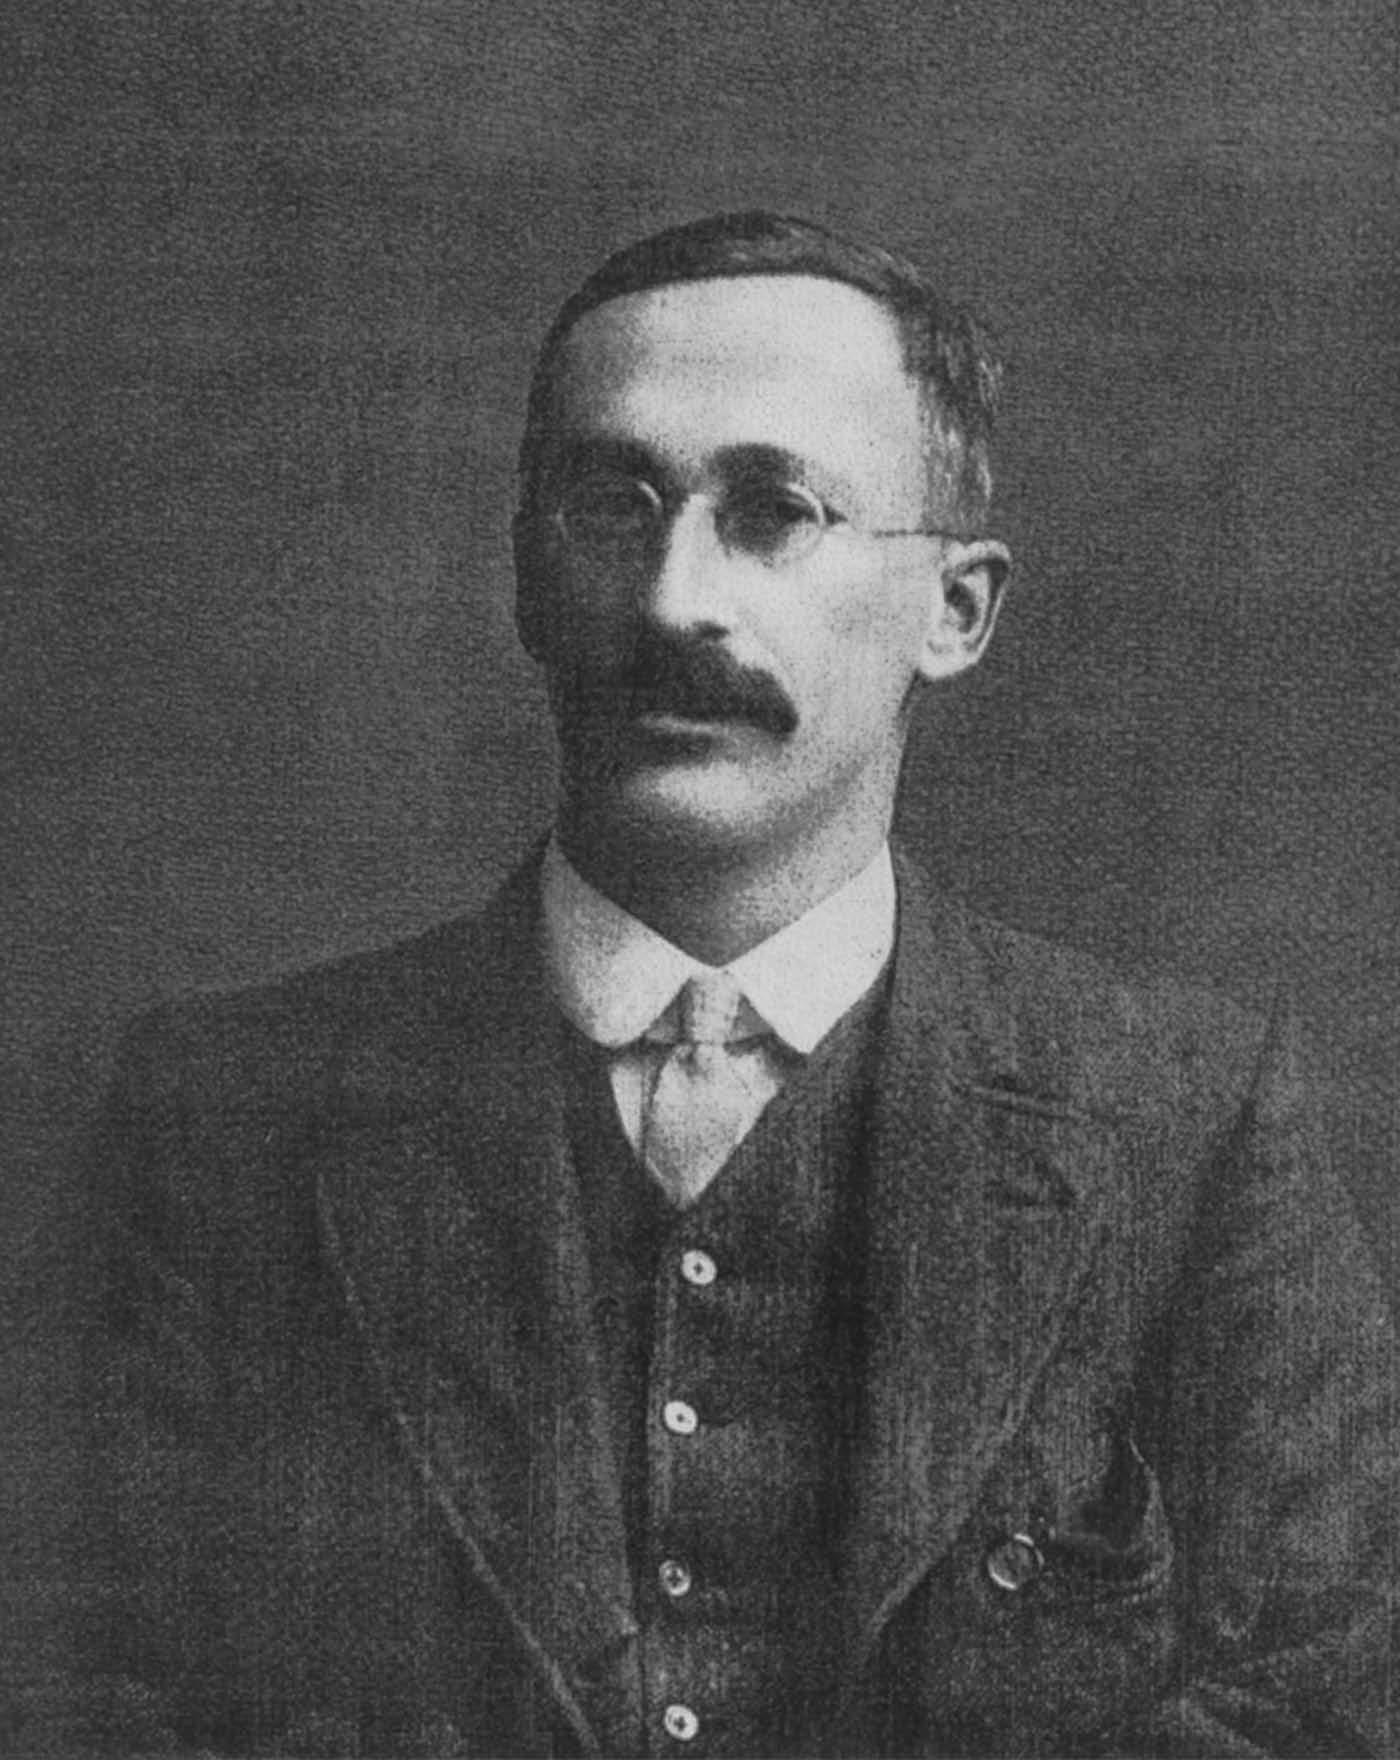
\includegraphics[scale = 0.05]{./images/gosset}}
\vspace{0.75em}


\includegraphics[scale = 0.17]{./images/guinness}
\end{figure}


\column{0.7\textwidth}
\footnotesize
\begin{quote}
``Student'' is the pseudonym used in 19 of 21 published articles by William Sealy
Gosset, who was a chemist, brewer, inventor, and self-trained statistician, agronomer, and designer of experiments ... [Gosset] worked his entire adult life ... as an experimental brewer for one employer: Arthur Guinness, Son \& Company, Ltd., Dublin, St.\ James’s Gate. Gosset was a master brewer and rose in fact to the top of the top of the brewing industry: Head Brewer of Guinness.
\end{quote}

\end{columns}

\end{frame}

%%%%%%%%%%%%%%%%%%%%%%%%%%%%%%%%%%%%%%%%

\begin{frame}
\frametitle{CI for Mean of Normal Distribution, Popn.\ Var.\ Unknown}
Same argument as we used when the variance was known, except with $t(n-1)$ rather than standard normal distribution:
	\begin{eqnarray*}
		P\left(-c \leq \frac{\bar{X}_n-\mu}{S/\sqrt{n}} \leq c \right) &=& 1-\alpha \\ \\ 
		P\left(\bar{X}_n - c \frac{S}{\sqrt{n}} \leq \mu\leq \bar{X}_n +c \frac{S}{\sqrt{n}} \right) &=& 1-\alpha 
	\end{eqnarray*}

\alert{$c =$ \texttt{qt}$(1-\alpha/2, \texttt{df} = n-1)$} 
	$$\boxed{\bar{X}_n \pm \texttt{qt}(1-\alpha/2, \texttt{df} = n-1)\;  \frac{S}{\sqrt{n}}}$$
\end{frame}



%%%%%%%%%%%%%%%%%%%%%%%%%%%%%%%%%%%%%%%%
\begin{frame}
\frametitle{Comparison of CIs for Mean of Normal Distribution}
\framesubtitle{$100\times(1-\alpha)\%$ Confidence Level}
$$\boxed{X_1, \hdots, X_n \sim \mbox{iid } N(\mu, \sigma^2)}$$


\begin{block}{Known Population Std.\ Dev.\ ($\sigma$)}
	$$\bar{X}_n \pm \; \texttt{qnorm}(1-\alpha/2) \; \frac{\sigma}{\sqrt{n}}$$
\end{block}


\begin{block}{Unknown Population Std.\ Dev.\ ($\sigma$)}
$$\bar{X}_n \pm \; \texttt{qt}(1-\alpha/2, \texttt{df} = n-1) \; \frac{S}{\sqrt{n}}$$
\end{block}
\end{frame}
%%%%%%%%%%%%%%%%%%%%%%%%%%%%%%%%%%%%%%%%
\begin{frame}
\frametitle{Standard Error vs.\ Estimator of Standard Error}
\begin{block}{Standard Error}
Recall that the standard deviation of  the sampling distribution of an estimator is called the \emph{\alert{standard error} (SE)} of that estimator.
\end{block}
\begin{block}{Example: Standard Error of the Mean}
$SE(\bar{X}_n) = \sqrt{Var\left(\bar{X_n}\right)} = \sigma/\sqrt{n}$
\end{block}



\begin{alertblock}{Estimator of Standard Error of the Mean} Whereas $\sigma/\sqrt{n}$ \alert{\emph{is}} the standard error of the mean, $S/\sqrt{n}$ is an \alert{\emph{estimator}} of this quantity: $\widehat{SE}(\bar{X_n}) = S/\sqrt{n}$
\end{alertblock}
\end{frame}
%%%%%%%%%%%%%%%%%%%%%%%%%%%%%%%%%%%%%%%%
\begin{frame}
\frametitle{Writing the CIs in terms of Actual and Estimated SE}
\framesubtitle{$100\times(1-\alpha)\%$ Confidence Level}
$$\boxed{X_1, \hdots, X_n \sim \mbox{iid } N(\mu, \sigma^2)}$$

\begin{block}{Known Population Std.\ Dev.\ ($\sigma$)}
	$$\bar{X}_n \pm \; \texttt{qnorm}(1-\alpha/2) \; \alert{SE(\bar{X}_n)}$$
\end{block}

\begin{block}{Unknown Population Std.\ Dev.\ ($\sigma$)}
$$\bar{X}_n \pm \; \texttt{qt}(1-\alpha/2, \texttt{df} = n-1) \; \alert{\widehat{SE}(\bar{X}_n)}$$
\end{block}
\end{frame}
%%%%%%%%%%%%%%%%%%%%%%%%%%%%%%%%%%%%%%%%
\begin{frame}
\frametitle{Comparison of Normal and $t$ CIs}
\begin{table}
\caption{Values of \texttt{qt}$(1-\alpha/2, \texttt{df}=n-1)$ for various choices of $n$ and $\alpha$. }
\begin{tabular}{r|rrrrr|r}
\hline
$n$& 1& 5& 10& 30& 100 & $\infty$\\
\hline
$\alpha = 0.10$&  6.31& 2.02 & 1.81 & 1.70  & 1.66 &1.64\\
$\alpha = 0.05$ & 12.71& 2.57 & 2.23 & 2.04  & 1.98 &1.96\\
$\alpha = 0.01$ & 63.66& 4.03 & 3.17 & 2.75  & 2.63 &2.58\\
\hline
\end{tabular}
\end{table}
\alert{Recall that as $n\rightarrow \infty$, $t(n-1) \rightarrow N(0,1)$}
\vspace{1em}


In a sense, using the $t$-distribution involves making a ``small-sample correction.'' In other words, it is only when $n$ is fairly small that this makes a practical difference for our confidence intervals.
\end{frame}
%%%%%%%%%%%%%%%%%%%%%%%%%%%%%%%%%%%%%%%%


\begin{frame}
\frametitle{Am I Taller Than The Average American Male?}
\framesubtitle{\href{http://www.cdc.gov/nchs/data/series/sr_11/sr11_252.pdf}{\fbox{Source: Centers for Disease Control (pg.\ 16)}}}


\begin{columns}
\column{0.4\textwidth}
\footnotesize
		\begin{tabular}{|lr|}
		\hline
			Sample Mean & 69 inches\\
			Sample Std.\ Dev.\ & 6 inches\\
			Sample Size & 5647 \\
			\hline
			My Height & 73 inches\\
			\hline
		\end{tabular}

\begin{eqnarray*}
\widehat{SE}(\bar{X}_n) &=& s/\sqrt{n}\\
	& =& 6/\sqrt{5647}\\ 
	&\approx& 0.08
\end{eqnarray*}


\column{0.6\textwidth}
Assuming the population is normal,\\
$\boxed{\bar{X}_n \pm \; \texttt{qt}(1-\alpha/2, \texttt{df} = n-1) \; \widehat{SE}(\bar{X}_n)}$
	

\vspace{1em}
\alert{What is the approximate value of \texttt{qt(1-0.05/2, df = 5646)}?} \pause


\vspace{1em}
For large $n$, $t(n-1) \approx N(0,1)$, so the answer is approximately 2
\pause

 \vspace{1em}
\alert{What is the ME for the 95\% CI?} 

\pause $ME \approx 0.16 \implies69 \pm 0.16$

\end{columns}
 


\end{frame}
%%%%%%%%%%%%%%%%%%%%%%%%%%%%%%%%%%%%%%%%
